\section{Adding images: \addbs{tkzTabIma} and \addbs{tkzTabImaFrom}}
These macros place a value on an arrow of the line of variations. A value can only be placed on an interval where the function is \tkzname{monotonic}, and the image is the image of a value already given in the first row. The first macro is \tkzcname{tkzTabIma}.

\subsection{Definition of \addbs{tkzTabIma}}

\begin{NewMacroBox}{tkzTabIma}{\oarg{local options}\{Begin\}\{End\}\{Position\}\{Image\}}

\begin{tabular}{lllc}
\toprule
\texttt{arguments}   & \texttt{default}    & \texttt{definition}                        \\
\toprule
\IargName{tkzTabIma}{Begin} & |no default|& rank of the start of the arrow      \\
\IargName{tkzTabIma}{End}  & |no default|& rank of the end of the arrow   \\
\IargName{tkzTabIma}{Position} & |no default| & rank of the value whose image is placed      \\
\IargName{tkzTabIma}{Image}     & |no default|  & value of the image     \\
\bottomrule
\end{tabular}

\medskip
\noindent\emph{Some comments: the first thing is to choose the arrow on which the image is placed. \tkzname{Begin} and \tkzname{End} are the ranks of the values at the ends of the arrow. \tkzname{Image} is the value to place. \tkzname{Position} is an integer: the rank of the value of the variable.}

\medskip
\begin{tabular}{lllc}
\toprule
\texttt{options}   & \texttt{default}    & \texttt{definition}                                      \\
\midrule
\IoptName{tkzTabIma}{draw}    & |false|   & draws an arrow from the value to its image     \\
\IoptName{tkzTabIma}{remember}& |lastval|& gives a name to the node of the image                   \\
\bottomrule
\end{tabular}

\medskip
\noindent\emph{For an arrow from the value to its image, use the option \tkzname{draw}. To refer later to the point where the image is, use the option \tkzname{remember}.}
\end{NewMacroBox}

\subsubsection{Adding the image of a given value}
There are several ways, but this one is the best. The value has rank $2$.
 The function is monotonic between the values of rank $1$ and $3$. Here is how to show the image of $\sqrt\E$ by $f$.

\begin{tkzexample}[vbox,small]
\begin{tikzpicture}
\tkzTabInit[espcl=6]%
  {$x$/1,$f'(x)$/1, $f(x)$/2}{$0$,$\sqrt\E$,$+\infty$}%
 \tkzTabLine{d,+,0,+,}%
 \tkzTabVar{D- /$-\infty$ , R /    ,+ / $0$ }%
 \tkzTabIma{1}{3}{2}{-5}
\end{tikzpicture}
\end{tkzexample}
\Iopt{tkzTabVal}{draw}

Another way is to use the macro \tkzcname{tkzTabImaFrom} with the nodes created to build the table; see the section ``Customizing the tables'' (\ref{pers}) and the end of this section.

\subsubsection{Example with several lines of variations}
\begin{tkzexample}[vbox,small]
	\begin{tikzpicture}

	  \tkzTabInit[espcl=4]
	     { $x$                     /1,
	       $f''(x)$                /1,
	       $f'$                     /2,
	        Sign of\\ $f'(x)$      /2,
	       $f$                     /3}%
	     { $0$      , $1$ ,     $\alpha$,$+\infty$ }%
	  \tkzTabLine {d    , + ,   z  , -  ,      , -  }%
	  \tkzTabVar
	      {- / $1$       ,
	       + /           ,
	       R /           ,
	       - / $-\infty$ }
	  \tkzTabIma[draw]{2}{4}{3}{$0$}
    % or \tkzTabVal[draw]{2}{4}{0.5}{}{0} (obsolete)
    	  \tkzTabLine {     , + ,      , +  ,  z   , -  }%
	  \tkzTabVar
	     {- / $-\infty$ ,
	      R /     ,
	      + / $1$ ,
	      - / $0$       }
	  \tkzTabIma[draw]{1}{3}{2}{$0$}
	\end{tikzpicture}
\end{tkzexample}


\subsubsection{Parametric functions}
\NameFonct{Parametric functions}

\begin{tkzexample}[vbox,small]
  \begin{tikzpicture}
  \tkzTabInit[ lgt=4,  deltacl=1, espcl=2]%
    {$t$                             /1,
    Sign of\\      $x'(t)$          /1.5,
    Variations of\\ $x$              /3,
     Variations of\\  $y$            /3,
    Sign of\\ $y'(t)$              /1.5}
    { $-\infty$ , $-4$ , $-1$ , $0$, $2$ , $+\infty$}%

  \tkzTabLine { , - , z , + , d , + , z , - , d , - , }

  \tkzTabVar  {+/$1$ , -/$ \frac{8}{9}$ ,+D-/$+\infty$/$-\infty$ ,
               +/$0$/ ,-D+ /$-\infty$/ $+\infty$ , -/$1$ /   }

  \tkzTabVar  {+/$+\infty$ , R/ ,-D+/$-\infty$/$+\infty$ ,
               -/$0$ ,R / , +/$+\infty$ }

  \tkzTabIma{1}{3}{2}{$\frac{32}{3}$}
  \tkzTabIma{4}{6}{5}{$\frac{16}{3}$}

  \tkzTabLine{ , - , \frac{-64}{9} , - , d , - , z , + , \frac{44}{9} , + , }
 \end{tikzpicture}
\end{tkzexample}

\subsection{Definition of \addbs{tkzTabImaFrom}}
This macro is like the previous one, but it places an image relative to another image, or relative to any named point of the table.

\begin{NewMacroBox}{tkzTabImaFrom}{\oarg{local options}\{Begin\}\{End\}\{From\}\{Image\}}

\begin{tabular}{lllc}
\toprule
\texttt{arguments}   & \texttt{default}    & \texttt{definition}                 \\
\midrule
\IargName{tkzTabImaFrom}{Begin}  & |no default|  & rank of the start of the arrow       \\
\IargName{tkzTabImaFrom}{End}  & |no default|  & rank of the end of the arrow     \\
\IargName{tkzTabImaFrom}{From}  & |no default|  & name of a point      \\
\IargName{tkzTabImaFrom}{Image}  & |no default|  & value of the image     \\
\bottomrule
\end{tabular}

\medskip
\noindent\emph{As for \tkzcname{tkzTabVal}, \tkzname{Begin} and \tkzname{End} are the ranks of the values at the ends of the arrow. \tkzname{Image} is the value to place. \tkzname{From} is the name of the node that corresponds to the value of the variable.}

\medskip
\begin{tabular}{lllc}
\toprule
\texttt{options}   & \texttt{default}    & \texttt{definition}                                     \\
\midrule
\IoptName{tkzTabImaFrom}{draw}    & |false|   & draws an arrow from the value to its image     \\
\IoptName{tkzTabImaFrom}{remember}& |lastval|& gives a name to the node of the image     \\
\bottomrule
\end{tabular}

\medskip
\noindent\emph{For an arrow from the value to its image, use the option \tkzname{draw}. To refer later to the point where the image is, use the option \tkzname{remember}.}

\end{NewMacroBox}

\subsubsection{Using a node defined by the macro \addbs{tkzTabInit}}
Here the node is \tkzname{N21}: a point below the second value $\sqrt\E$, on the first horizontal rule below this value. See the section \tkzname{Customizing the tables}, and in particular the option \tkzname{help}, which shows the construction points.

\begin{tkzexample}[vbox,small]
\begin{tikzpicture}
\tkzTabInit[espcl=6]%
  {$x$/1,$f'(x)$/1, $f(x)$/3}{$0$,$\sqrt\E$,$+\infty$}%
 \tkzTabLine{d,+,0,+,}%
 \tkzTabVar{D-/      $-\infty$, R/      , +/$0$   }
 \tkzTabImaFrom[draw]{1}{3}{N21}{-5}
 \draw[opacity=0.4,fill=red!30]  (N21) circle(3ex);
 \draw[fill=red]  (N21) circle(2pt);
 \node[above right= 12pt,red](txt) at (N21) {$N21$};
\end{tikzpicture}
\end{tkzexample}
\Iopt{tkzTabImaFrom}{draw}

\subsubsection{Using a point named by the user with \texttt{\textcolor{red}{remember}}}

\begin{tkzexample}[vbox, num,small]
	\begin{tikzpicture}
	\tkzTabInit[lgt=3,espcl=6]{ $x$/1, $f'(x)$/1, $f(x)$/3,/3 }%
	           {  $a$    , $d$    ,$e$}
	\tkzTabLine{  z,+    ,z,-     ,z  }
	\tkzTabVar  {-/\va  ,+/\vd   , -/  \ve}
	\tkzTabVal[draw,remember=vb]{1}{2}{0.333}{b}{$0$}
	\tkzTabVal[draw,remember=vc]{1}{2}{0.666}{c}{$1$}
	\tkzTabVar{-/\va  ,R/   , +/  \ve}
	\tkzTabVal[draw]{1}{3}{0.5}{}{$0$}
	\tkzTabImaFrom[draw]{1}{3}{vc}{$-1$}
	\tkzTabImaFrom[draw]{1}{3}{vb}{$-2$}
	\end{tikzpicture}
\end{tkzexample}
\Iopt{tkzTabImaFrom}{remember}

\endinput